%-*- coding: UTF-8 -*-
% gougu.tex
% 勾股定理


\documentclass[UTF8]{ctexart}
\usepackage{graphicx}
\usepackage{float}

\usepackage{amsmath}
\usepackage{cite}
\usepackage{geometry}
\usepackage{url}
\newcommand{\upcite}[1]{\textsuperscript{\textsuperscript{\cite{#1}}}}
\title{杂谈勾股定理}
\author{张三}
\date{\today}
\bibliographystyle{unsrt}
\newtheorem{thm}{定理}

\begin{document}

\maketitle
\tableofcontents
\section{勾股定理在古代}

西方称勾股定理为毕达哥拉斯定理,将勾股定理的发现归功于公元前6世纪的
毕达哥拉斯学派\upcite{Kline}。该学派得到了一个法则,可以求出可排成直角三角形三边的三
元数组。毕达哥拉斯学派没有书面著作,该定理的严格表述和证明则见于欧几里
德《几何原本》的命题␣47:“直角三角形斜边上的正方形等于两直角边上的两
个正方形之和。”证明是用面积做的。

\par
我国《周髀算经》载商高(约公元前12世纪)答周公问:
\begin{quote}
    \zihao{-5}\kaishu 勾广三,股修四,径隅五。
\end{quote}
又载陈子(约公元前7-6世纪)答荣方问:
\begin{quote}
    \zihao{-5}\kaishu 若求邪至日者,以日下为勾,日高为股,勾股各自乘,并而开方除之,得邪至日。
\end{quote}
都较古希腊更早。后者已经明确道出勾股定理的一般形式。图是我国古代对勾股定理的一种证明\upcite{quanjing}

\begin{figure}[ht]
    \centering
    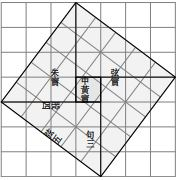
\includegraphics[width=3cm]{xiantu.JPG}
    \caption{\small\it 宋赵爽在《周髀算经》注中作的弦图(仿制),该图给出了勾股定理的极具对称美的证明。}
    \label{fig:gougudingli}
\end{figure}

\section{勾股定理的近代形式}


\begin{thm}[勾股定理]
    直角三角形斜边的平方等于两腰的平方和。
    可以用符号语言表述为:设直角三角形ABC,其中\angle C=$90^\circ$,则有
    \begin{equation}\label{eq:gougu}
         AB^2=BC^2+AC^2
    \end{equation}
\end{thm}


满足式的整数称为。第节所说毕达哥拉斯学派得到的三元数组就是勾股数。下表列出了一些较小的勾股数:\upcite{timmurphy.org}


\begin{table}[H]
    \begin{tabular}{|rrr|}
        \hline
        直角边$a$  &  直角边$b$  &  直角边$c$\\
        \hline
        3&4&5\\
        5&12&13\\\hline
    \end{tabular}%
    \qquad
    ($a^2 + b^2 = c^2$)
\end{table}


\nocite{Shiye}
\bibliography{math}

\end{document}